%!TEX root = ../paper.tex

\subsection{Risk and Benefit Rankings} 
%\begin{figure}[t]
%	\centering
%	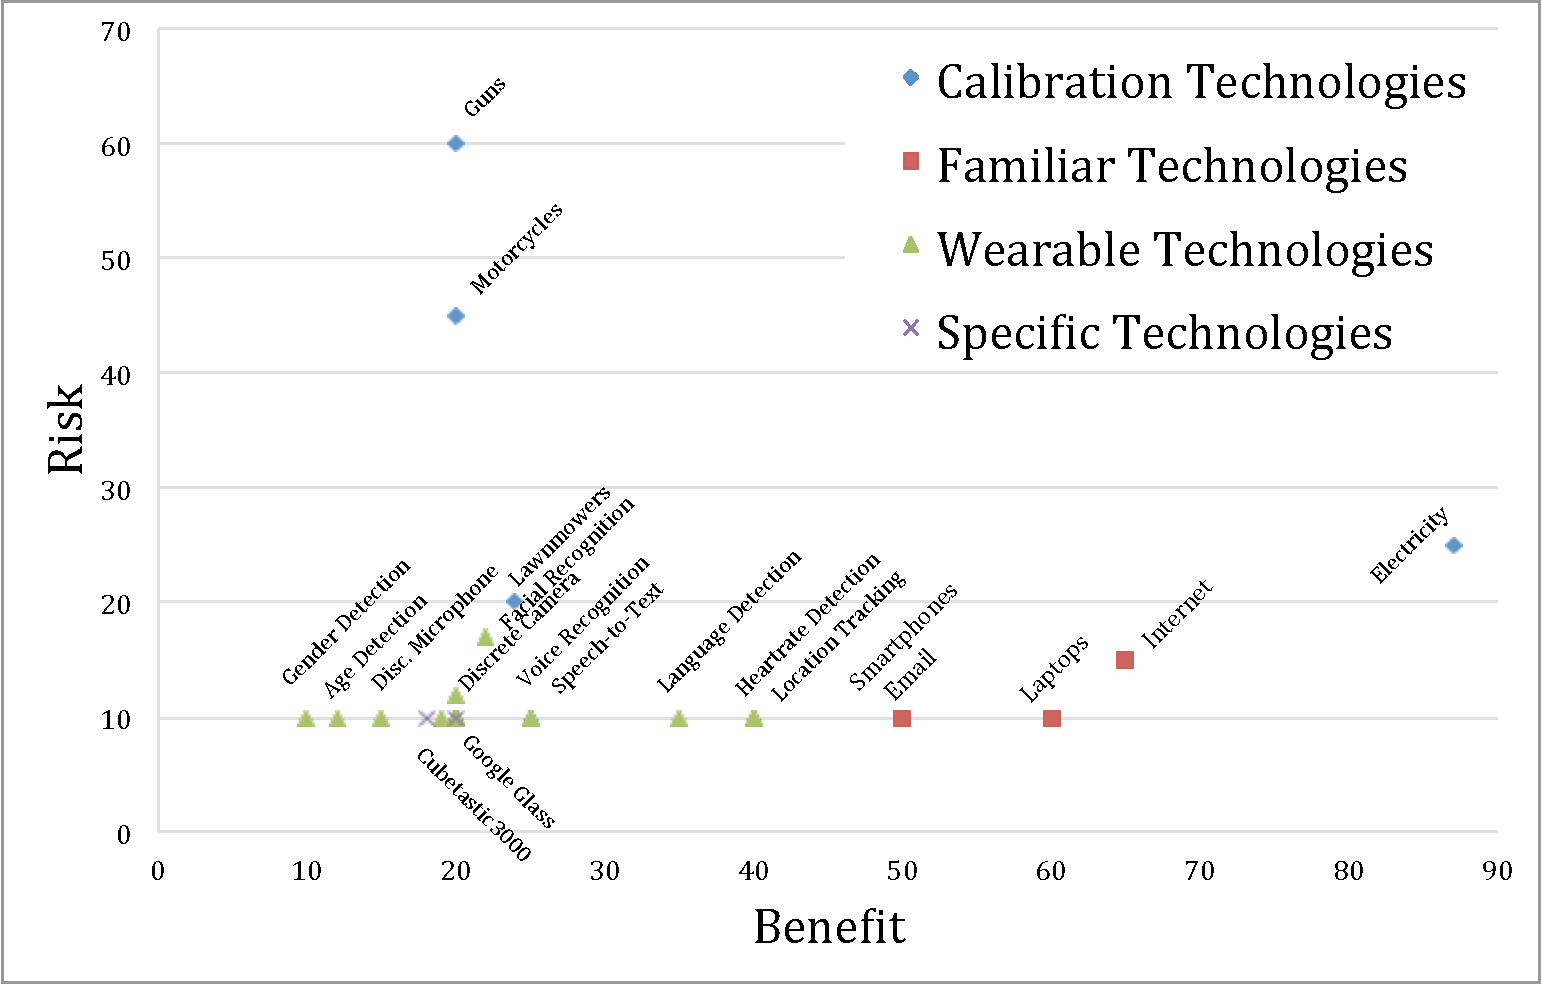
\includegraphics[width=0.47\textwidth]{images/riskbenefit.pdf}
%	\caption{Participants' median risk-benefit ratings of technologies examined by Fischhoff \etal\cite{Fischhoff}, which we used for calibration, alongside familiar technologies (e.g., laptops, the Internet, etc.), wearable technologies, as well as two specific wearable devices (Google Glass and the Cubetastic3000).}
%	\label{fig:techplot}
%\end{figure}

We asked participants to rate new capabilities related to wearable technologies (e.g., facial recognition) in terms of their risks and benefits. We also asked them to do this for technologies with which they were likely to be more familiar (e.g., smartphones and laptops) in addition to two examples of specific wearable devices, Google Glass and the fictitious Cubetastic3000. To calibrate our results, we also asked about four well-established technologies studied by Fischhoff \etal\cite{Fischhoff}. We found that participants generally rated familiar technologies and those related to wearables as being low-risk. Figures ~\ref{risk, benefit} depicts participants' median ratings. We found that the calibration technologies were all rated as the most risky. At the same time, with the exception of electricity, the calibration technologies were seen as lower benefit than the others.

As a group, participants rated the familiar technologies as the most beneficial. We believe this is the result of exposure people have to these technologies---most people use these technologies daily. Of the wearable technologies, the most risky were ones perceived to be privacy-invasive; the most risky technologies were facial recognition, the Internet, and discrete cameras, whereas the remainder of the technologies were seen as having minimal---albeit equivalent---risk levels (i.e., a median of ``10''). People are becoming increasingly aware of such privacy risks and are comparing these privacy invasion to real physical risks--for instance, the capacity for facial detection on a wearable device is perceived to be almost as risky as interacting with a lawnmower.

{\color {red} talk about the distributions and variance of the particular technologies, referring to the table in the appendix}

{\color {red} people may have evaluated the risks only thinking of physical risk, not privacy risk. This might have happened because among the 5 presented options, the wearable-related one is the odd one out; all other options involve some physical risk scenario. These other options, by being the most prominent (4 versus 1), frame the risk perception in the user's mind as meaning "physical risk", and users may consequently ignore or downplay privacy risks. It would have been better to ask 4+4  questions (or 2+2 to keep the survey short) rather than the current 4+1. AND "with the exception of electricity, the calibration technologies were seen as lower benefit than the others". This is true for some, but not all of the others. Specifically, Google glass and Cubetastic3000 were about equally beneficial, and gender and age recognition were less beneficial. AND The differences in risk that *are* found between the different wearable-related are not tested for statistical significance, but given their minimal spread compared to the calibration options, the differences are negligible.}

These perceptions of the most risky or beneficial technologies may not be reflective of actual risks or benefits. However, they do reflect the general public's exposure to these technologies and show that people perceive specific risks and benefits. We suspect that the similarity in assessments between the various wearable technologies are because most people are not consciously aware of the possibilities of these technologies or how they could be used. We suspect that performing this experiment longitudinally may yield more interesting results, as these technologies become more and more pervasive (and therefore more familiar to participants).

\begin{table}[t]
\begin{center}
\small
\begin{tabular}{| p{2cm} | p{1cm} | p{1cm} | p{1cm} | c |}
\hline
Technology & Q1 &  Median & Q3 & Distribution  \\ 
\hline
Location Tracking & 10.0 & 10.0 & 20.0 & 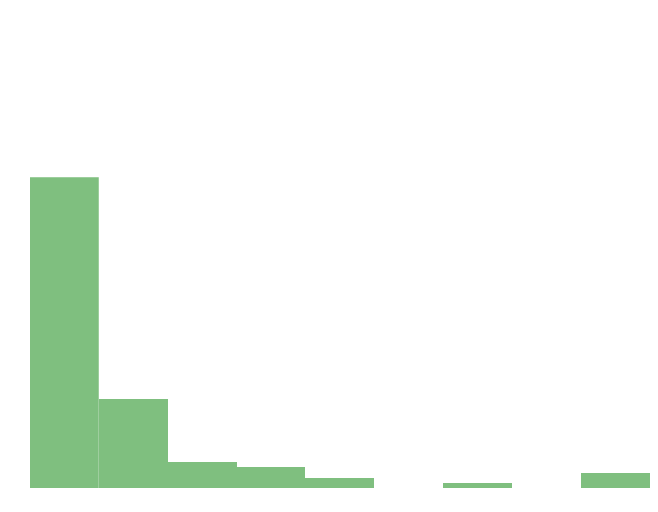
\includegraphics[width = 2cm, height = 0.5cm]{tex-inputs/table-images/locationtrackingrisk} \\ 
Speech To Text & 10.0 & 10.0 & 10.0 & 
\includegraphics[width = 2cm, height = 0.5cm]{tex-inputs/table-images/speechtotextrisk} \\ 
Discreet Microphone & 10.0 & 10.0 & 20.0 & 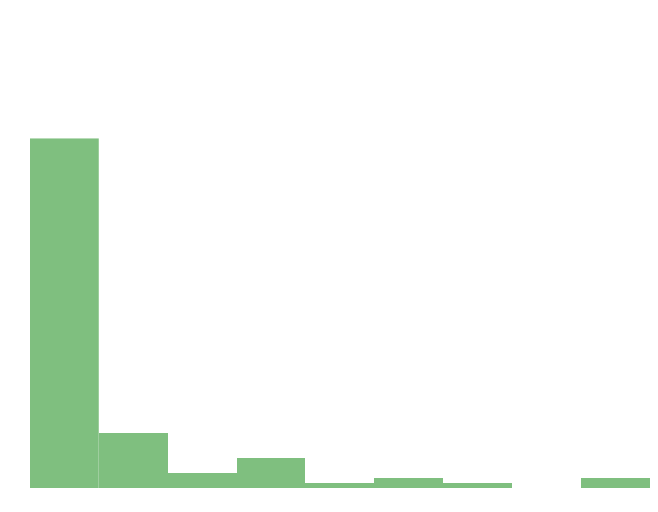
\includegraphics[width = 2cm, height = 0.5cm]{tex-inputs/table-images/discreetmicrophonerisk} \\ 
Smartwatches & 10.0 & 10.0 & 10.0 & 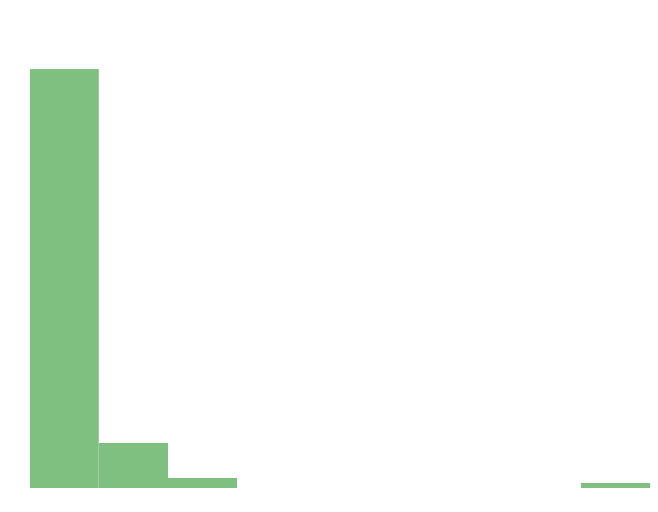
\includegraphics[width = 2cm, height = 0.5cm]{tex-inputs/table-images/smartwatchesrisk} \\ 
Language Detection & 10.0 & 10.0 & 10.0 & 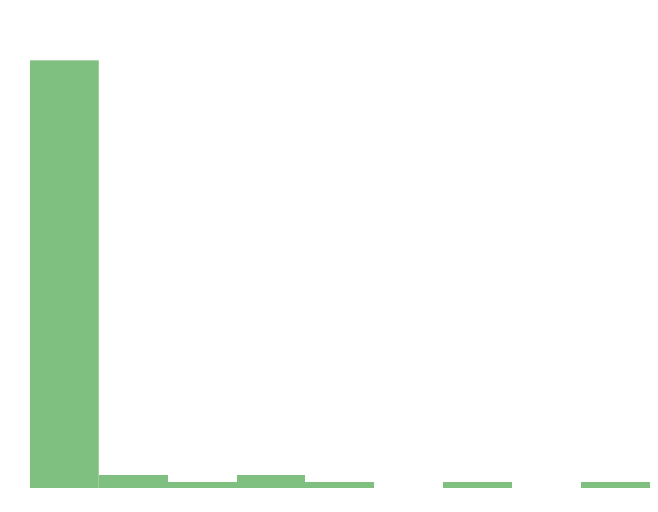
\includegraphics[width = 2cm, height = 0.5cm]{tex-inputs/table-images/languagedetectionrisk} \\ 
Laptops & 10.0 & 10.0 & 15.0 & 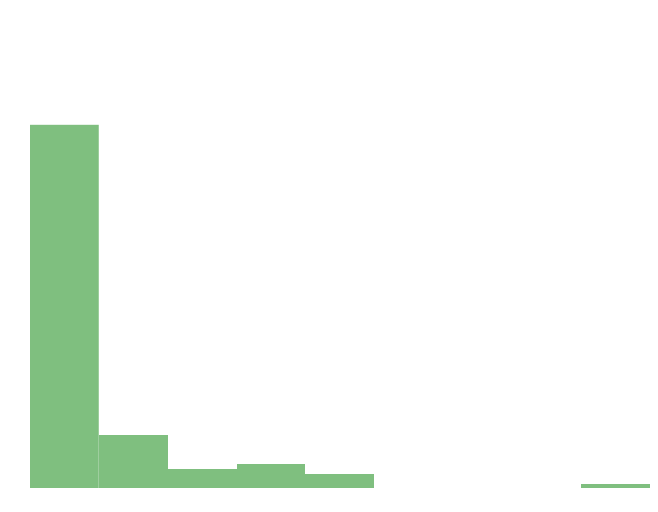
\includegraphics[width = 2cm, height = 0.5cm]{tex-inputs/table-images/laptopsrisk} \\ 
Smartphones & 10.0 & 10.0 & 20.0 & 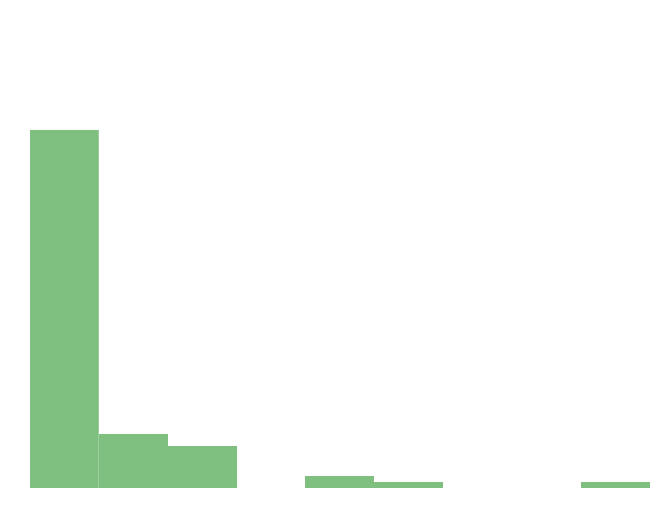
\includegraphics[width = 2cm, height = 0.5cm]{tex-inputs/table-images/smartphonesrisk} \\ 
Google Glass & 10.0 & 10.0 & 20.0 & 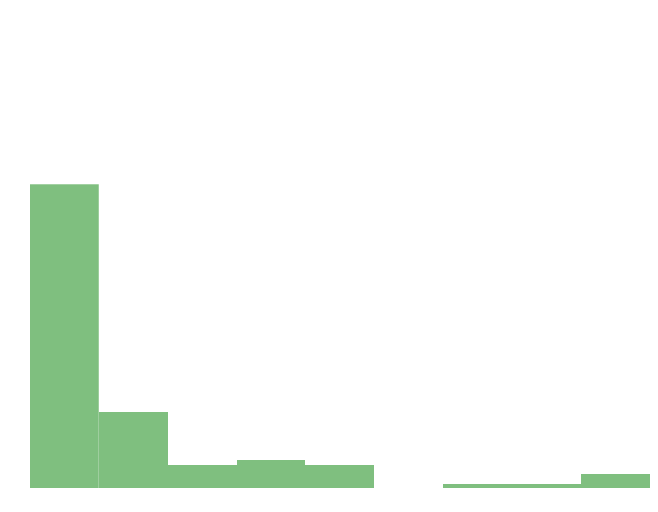
\includegraphics[width = 2cm, height = 0.5cm]{tex-inputs/table-images/googleglassrisk} \\ 
Cubetastic & 10.0 & 10.0 & 30.0 & 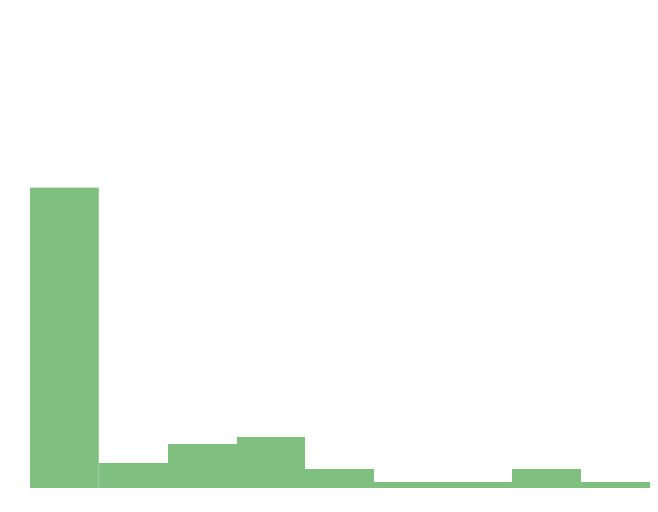
\includegraphics[width = 2cm, height = 0.5cm]{tex-inputs/table-images/cubetasticrisk} \\ 
Gender Detection & 10.0 & 10.0 & 13.5 & 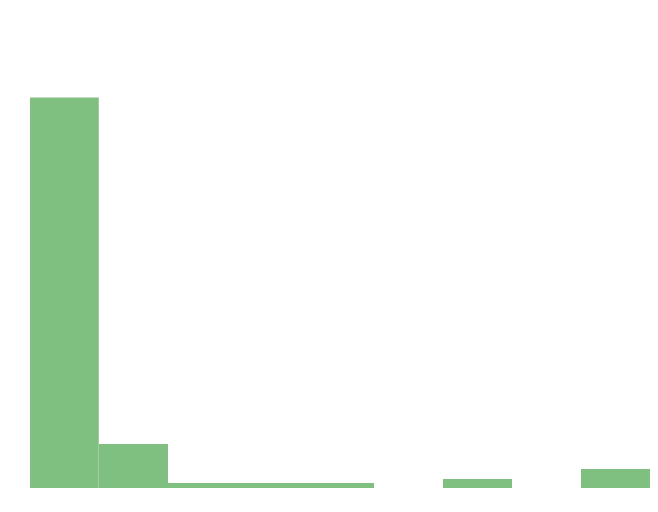
\includegraphics[width = 2cm, height = 0.5cm]{tex-inputs/table-images/genderdetectionrisk} \\ 
Voice Recognition & 10.0 & 10.0 & 15.0 & 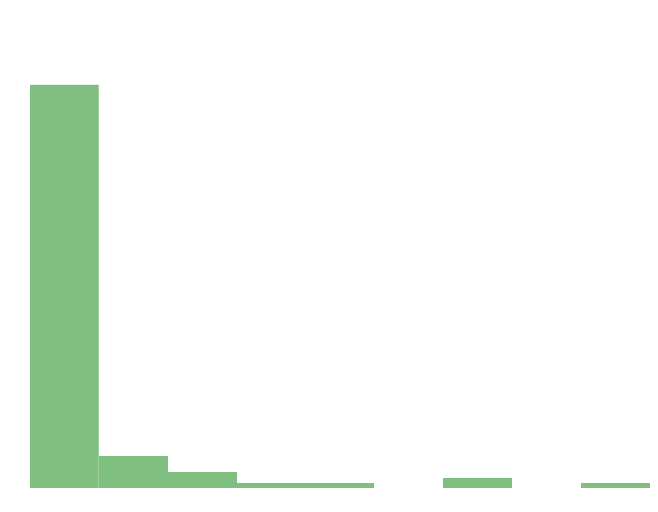
\includegraphics[width = 2cm, height = 0.5cm]{tex-inputs/table-images/voicerecognitionrisk} \\ 
Voice Based Emotion Detection & 10.0 & 10.0 & 15.0 & 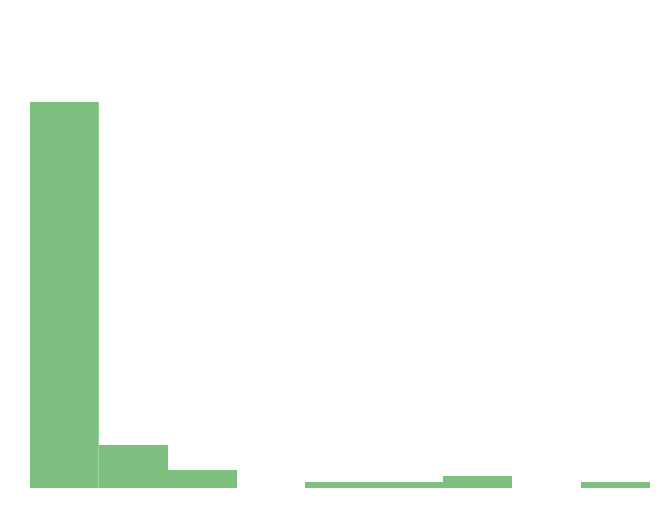
\includegraphics[width = 2cm, height = 0.5cm]{tex-inputs/table-images/voicebasedemotiondetectionrisk} \\ 
Fitness Trackers & 10.0 & 10.0 & 10.0 & 
\includegraphics[width = 2cm, height = 0.5cm]{tex-inputs/table-images/fitnesstrackersrisk} \\ 
Age Detection & 10.0 & 10.0 & 15.0 & 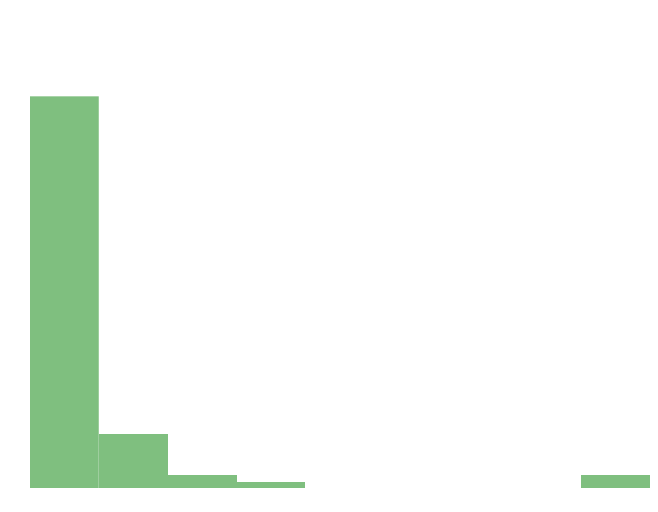
\includegraphics[width = 2cm, height = 0.5cm]{tex-inputs/table-images/agedetectionrisk} \\ 
Facial Detection & 10.0 & 10.0 & 25.0 & 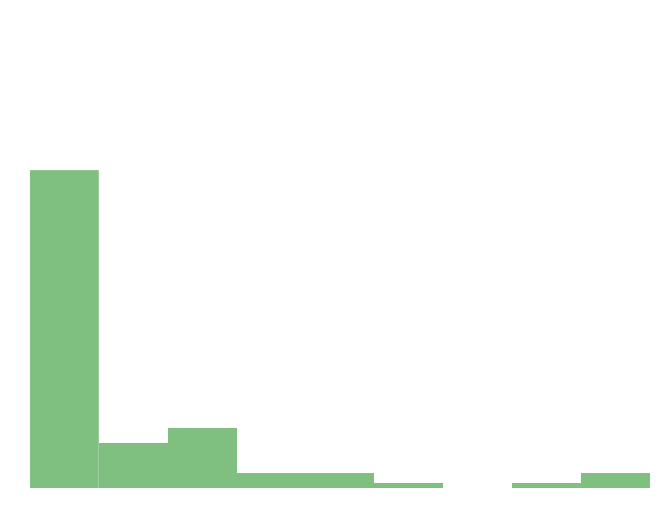
\includegraphics[width = 2cm, height = 0.5cm]{tex-inputs/table-images/facialdetectionrisk} \\ 
Email & 10.0 & 10.0 & 18.0 & 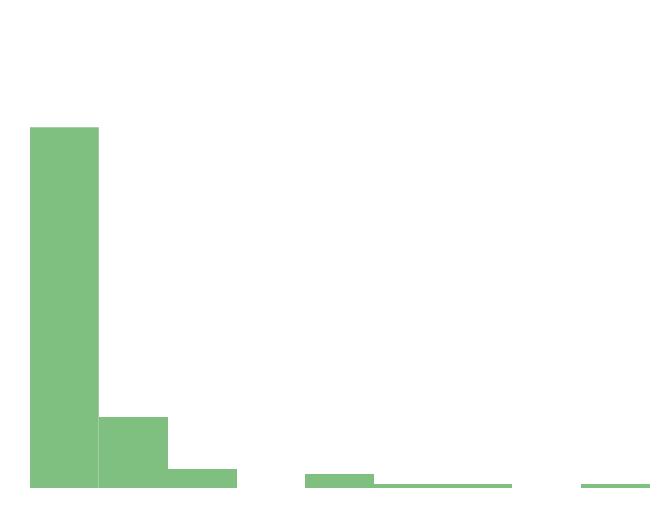
\includegraphics[width = 2cm, height = 0.5cm]{tex-inputs/table-images/emailrisk} \\ 
Heart Rate Detection & 10.0 & 10.0 & 10.0 & 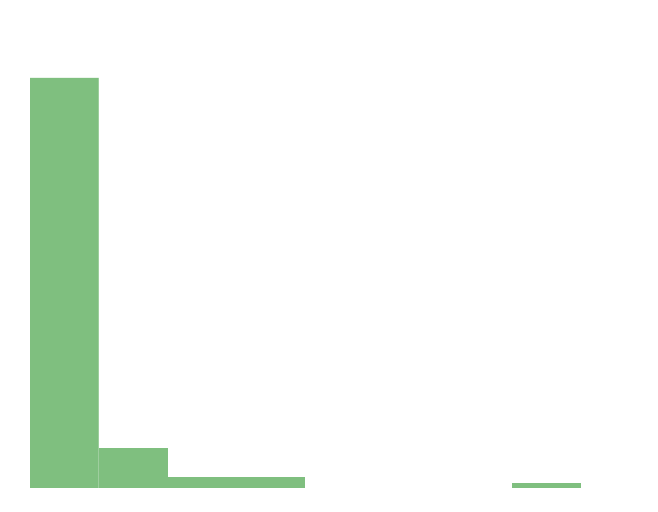
\includegraphics[width = 2cm, height = 0.5cm]{tex-inputs/table-images/heartratedetectionrisk} \\ 
Discreet Video Camera & 12.0 & 10.0 & 30.0 & 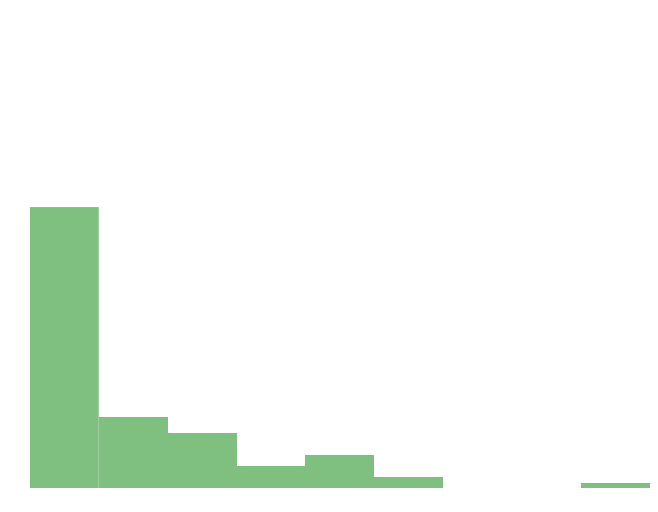
\includegraphics[width = 2cm, height = 0.5cm]{tex-inputs/table-images/discreetvideocamerarisk} \\ 
Internet & 15.0 & 10.0 & 31.0 & 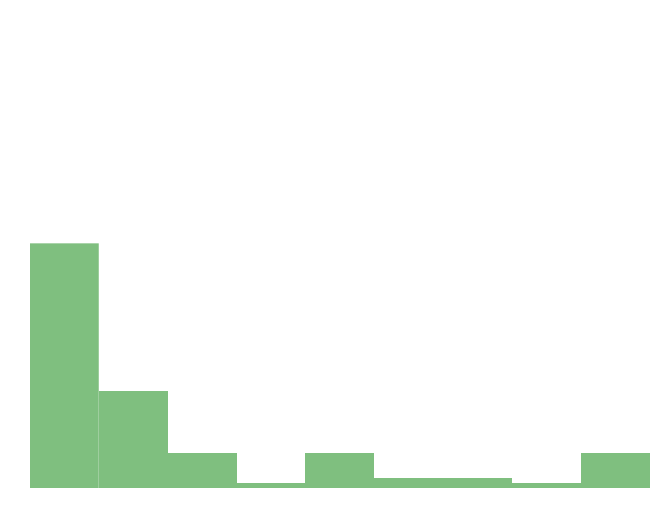
\includegraphics[width = 2cm, height = 0.5cm]{tex-inputs/table-images/internetrisk} \\ 
Facial Recognition & 17.0 & 10.0 & 30.0 & 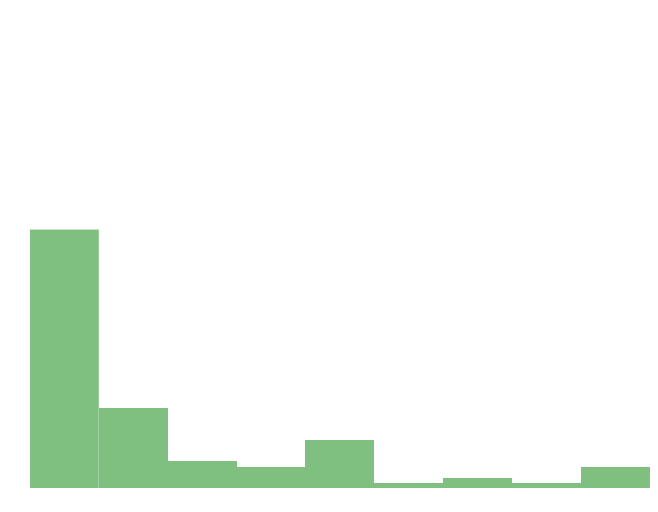
\includegraphics[width = 2cm, height = 0.5cm]{tex-inputs/table-images/facialrecognitionrisk} \\ 
Lawnmower & 20.0 & 12.0 & 30.0 & 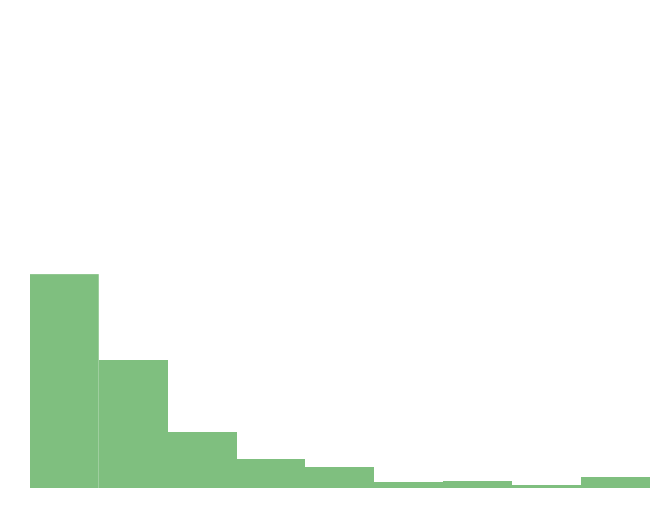
\includegraphics[width = 2cm, height = 0.5cm]{tex-inputs/table-images/LawnmowerRisk} \\ 
Electricity & 25.0 & 15.0 & 40.0 & 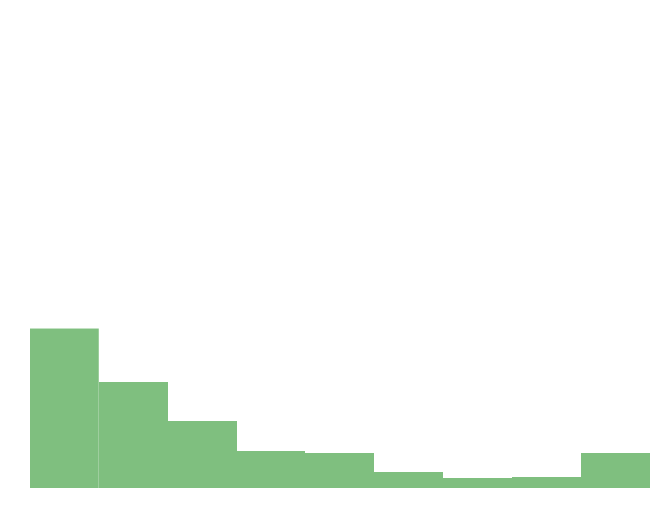
\includegraphics[width = 2cm, height = 0.5cm]{tex-inputs/table-images/ElectricityRisk} \\ 
Motorcycle & 45.0 & 27.0 & 70.0 & 
\includegraphics[width = 2cm, height = 0.5cm]{tex-inputs/table-images/MotorcycleRisk} \\ 
Handgun & 60.0 & 40.0 & 100.0 & 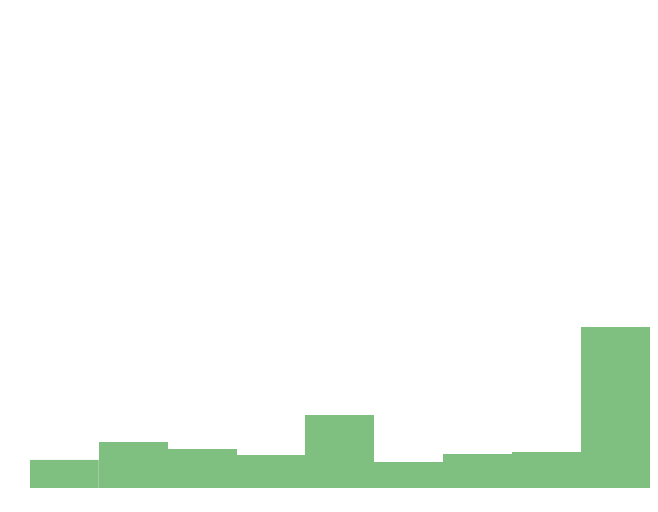
\includegraphics[width = 2cm, height = 0.5cm]{tex-inputs/table-images/HandgunRisk} \\ 
\hline
\end{tabular}
\caption{Risk rankings in response to the Fischoff-style prompt for various technologies and capabilities.Most technologies are capabilities with respect to wearable devices. Calibration technologies were electricity, guns, lawnmowers, and motorcycles. Wearable technologies included the Google Glass and the Cubetastic3000. Other specific technologies, such as internet, email, laptops, and smartphones, were also asked.}
\label{risk}
\end{center}
\end{table}

\begin{table}[t]
\begin{center}
\small
\begin{tabular}{| p{2cm} | p{1cm} | p{1cm} | p{1cm} | c |}
\hline
Technology & Q1 &  Median & Q3 & Distribution  \\ 
\hline
Gender Detection & 10.0 & 10.0 & 15.0 & 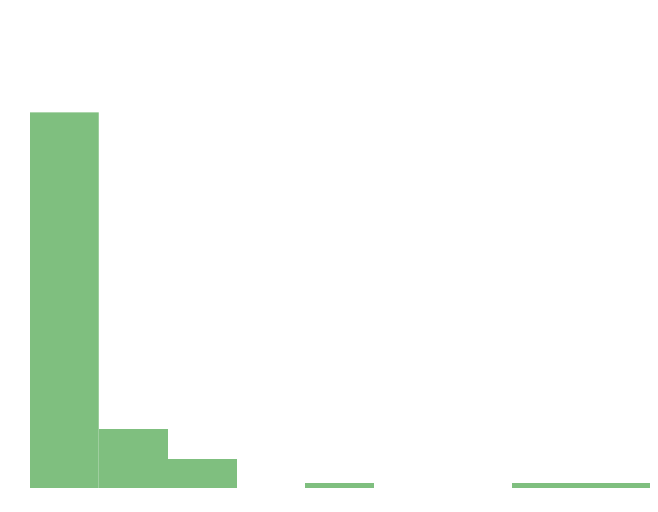
\includegraphics[width = 2cm, height = 0.5cm]{tex-inputs/table-images/genderdetectionben} \\ 
Age Detection & 12.0 & 10.0 & 22.0 & 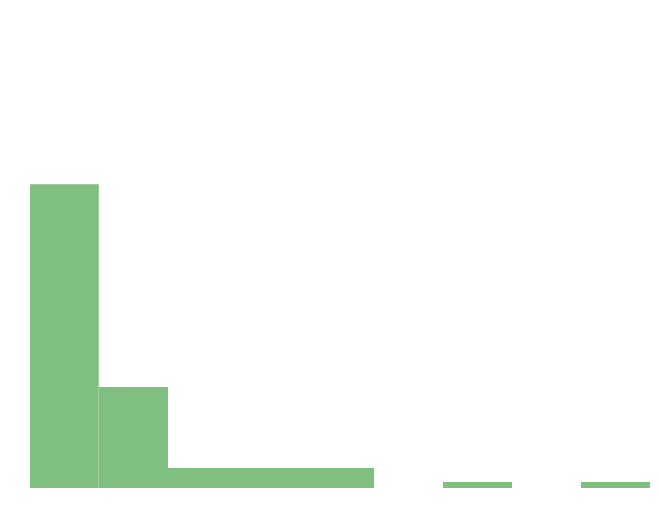
\includegraphics[width = 2cm, height = 0.5cm]{tex-inputs/table-images/agedetectionben} \\ 
Discreet Microphone & 15.0 & 10.0 & 20.0 & 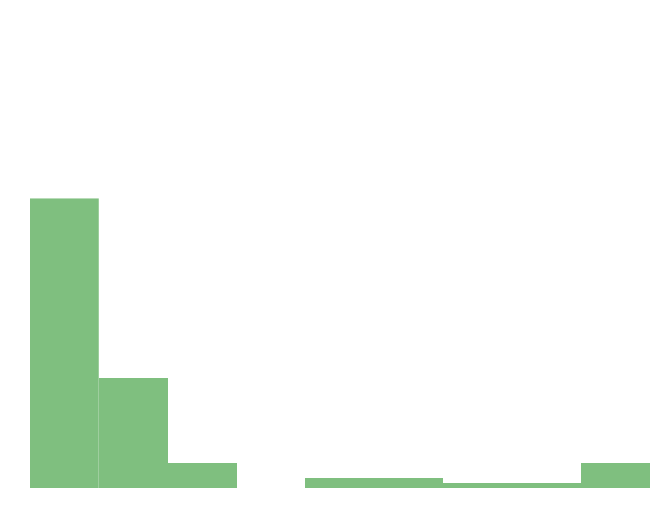
\includegraphics[width = 2cm, height = 0.5cm]{tex-inputs/table-images/discreetmicrophoneben} \\ 
Cubetastic & 15.0 & 10.0 & 30.0 & 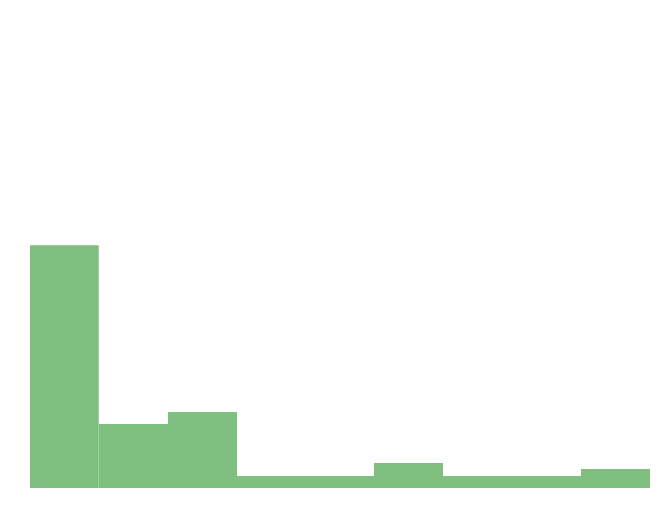
\includegraphics[width = 2cm, height = 0.5cm]{tex-inputs/table-images/cubetasticben} \\ 
Fitness Trackers & 18.5 & 10.0 & 30.0 & 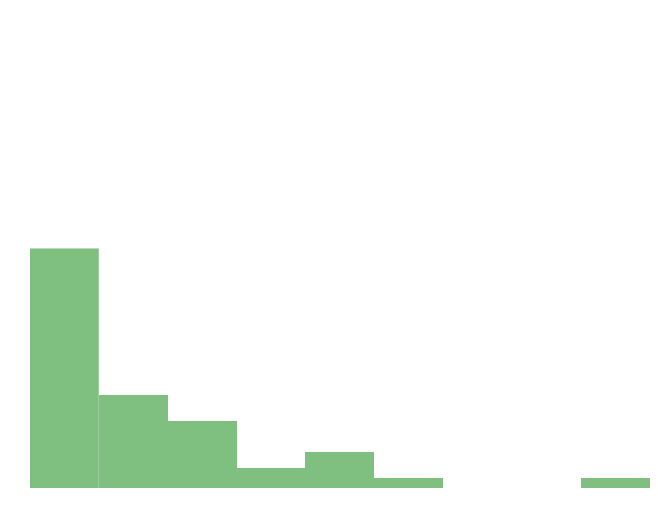
\includegraphics[width = 2cm, height = 0.5cm]{tex-inputs/table-images/fitnesstrackersben} \\ 
Voice Based Emotion Detection & 20.0 & 10.0 & 30.0 & 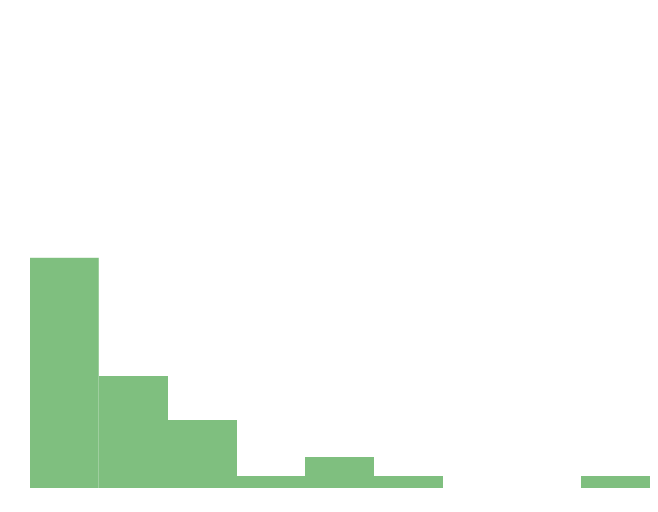
\includegraphics[width = 2cm, height = 0.5cm]{tex-inputs/table-images/voicebasedemotiondetectionben} \\ 
Facial Detection & 20.0 & 10.0 & 34.0 & 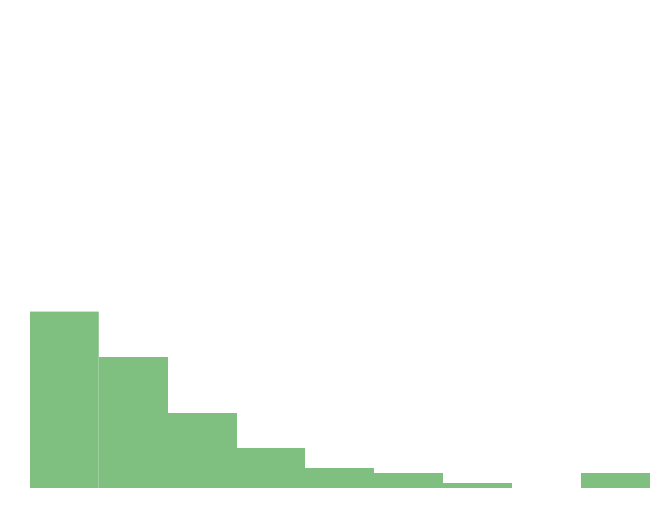
\includegraphics[width = 2cm, height = 0.5cm]{tex-inputs/table-images/facialdetectionben} \\ 
Discreet Video Camera & 20.0 & 15.0 & 30.0 & 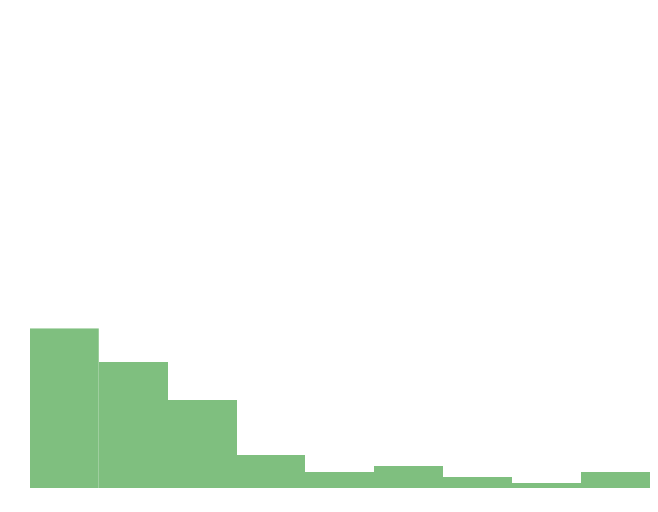
\includegraphics[width = 2cm, height = 0.5cm]{tex-inputs/table-images/discreetvideocameraben} \\ 
Google Glass & 20.0 & 12.0 & 40.0 & 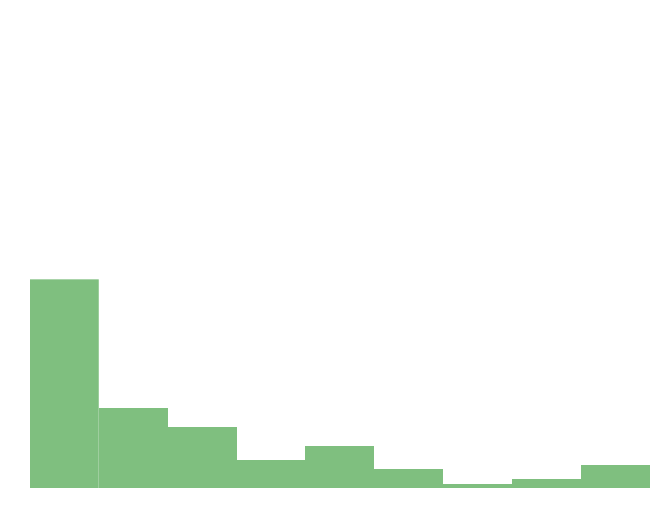
\includegraphics[width = 2cm, height = 0.5cm]{tex-inputs/table-images/googleglassben} \\ 
Smartwatches & 20.0 & 10.0 & 35.0 & 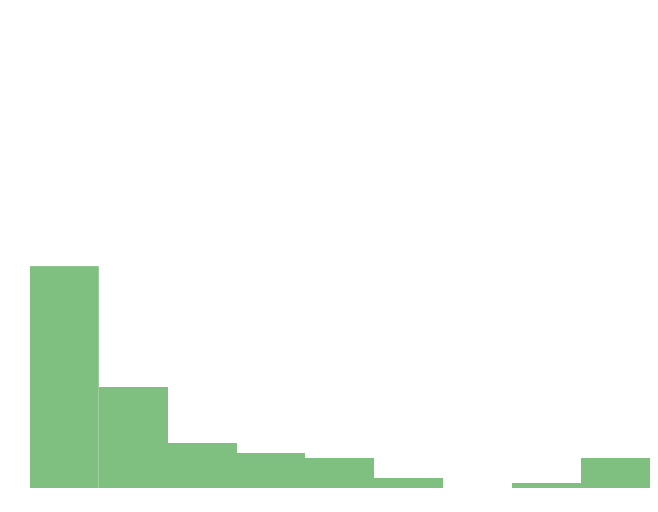
\includegraphics[width = 2cm, height = 0.5cm]{tex-inputs/table-images/smartwatchesben} \\ 
Motorcycle & 20.0 & 12.0 & 40.0 & 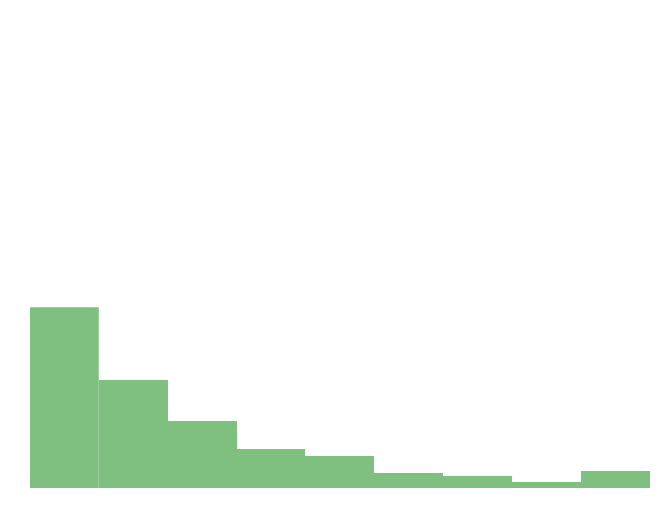
\includegraphics[width = 2cm, height = 0.5cm]{tex-inputs/table-images/MotorcycleBenefit} \\ 
Handgun & 20.0 & 10.0 & 30.0 & 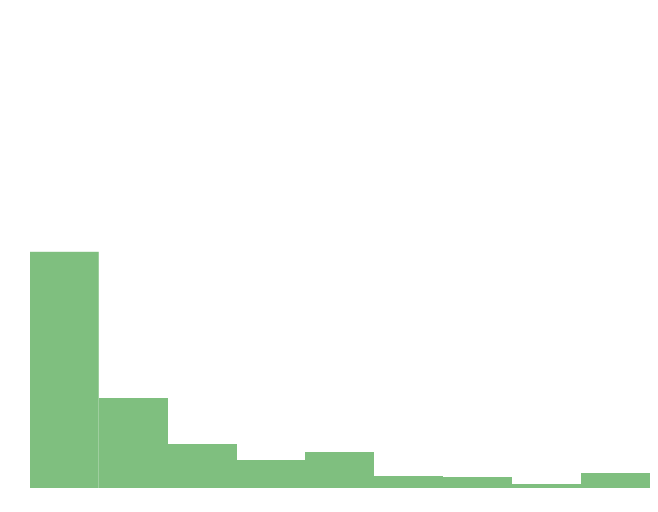
\includegraphics[width = 2cm, height = 0.5cm]{tex-inputs/table-images/HandgunBenefit} \\ 
Facial Recognition & 22.0 & 12.5 & 42.5 & 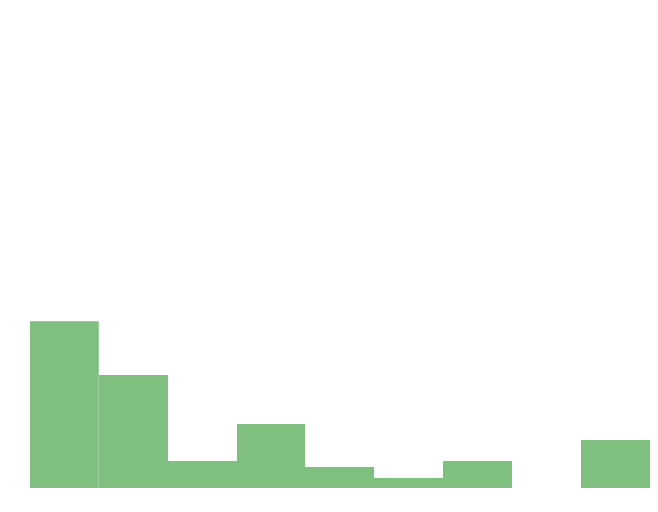
\includegraphics[width = 2cm, height = 0.5cm]{tex-inputs/table-images/facialrecognitionben} \\ 
Lawnmower & 24.0 & 15.0 & 40.0 & 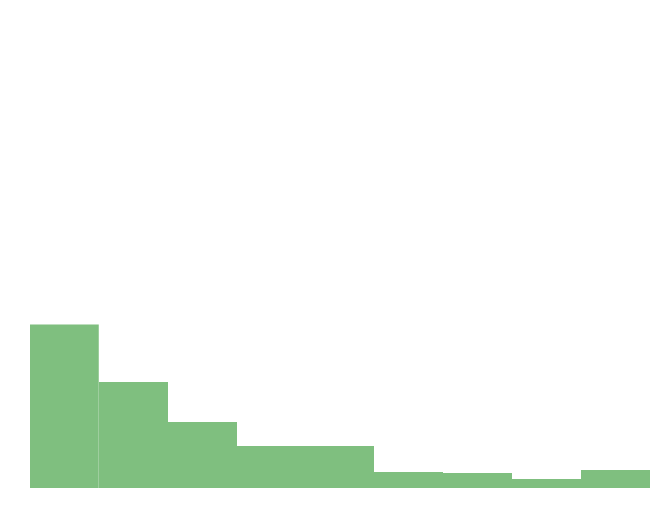
\includegraphics[width = 2cm, height = 0.5cm]{tex-inputs/table-images/LawnmowerBenefit} \\ 
Speech To Text & 25.0 & 15.0 & 40.0 & 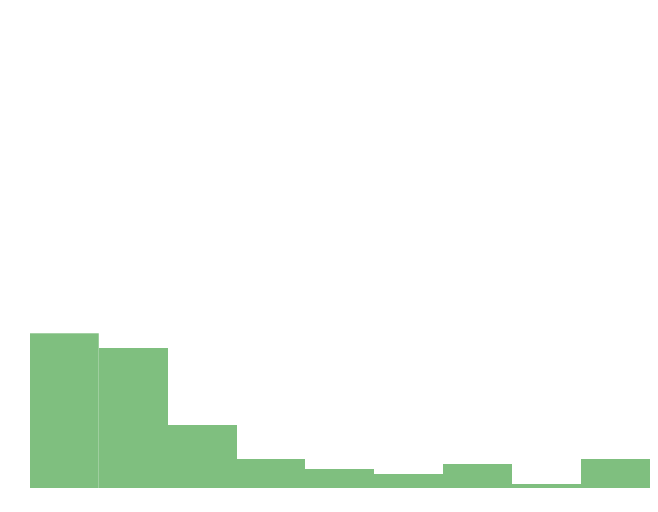
\includegraphics[width = 2cm, height = 0.5cm]{tex-inputs/table-images/speechtotextben} \\ 
Voice Recognition & 25.0 & 15.0 & 40.0 & 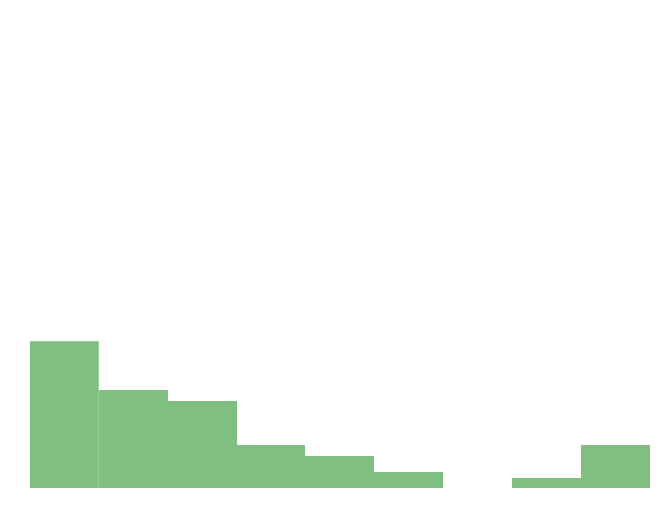
\includegraphics[width = 2cm, height = 0.5cm]{tex-inputs/table-images/voicerecognitionben} \\ 
Language Detection & 35.0 & 15.0 & 60.0 & 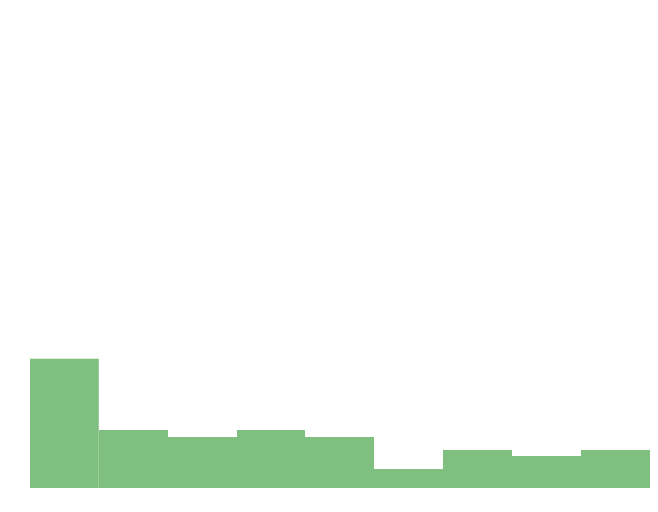
\includegraphics[width = 2cm, height = 0.5cm]{tex-inputs/table-images/languagedetectionben} \\ 
Heart Rate Detection & 40.0 & 26.0 & 65.0 & 
\includegraphics[width = 2cm, height = 0.5cm]{tex-inputs/table-images/heartratedetectionben} \\ 
Location Tracking & 40.0 & 20.0 & 70.0 & 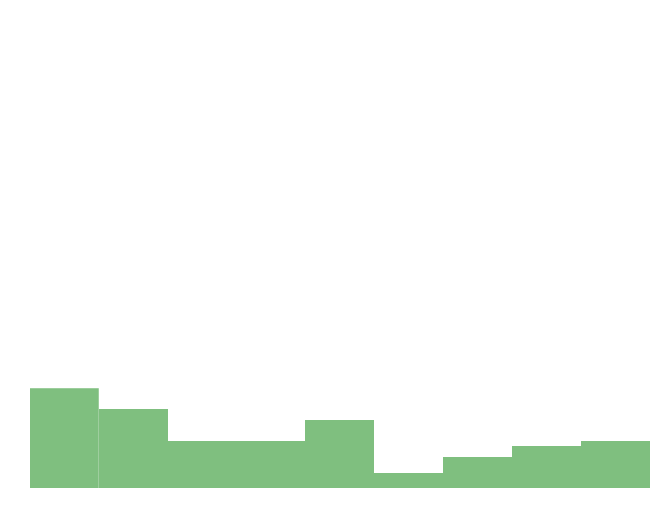
\includegraphics[width = 2cm, height = 0.5cm]{tex-inputs/table-images/locationtrackingben} \\ 
Email & 50.0 & 29.0 & 77.5 & 
\includegraphics[width = 2cm, height = 0.5cm]{tex-inputs/table-images/emailben} \\ 
Smartphones & 50.0 & 30.0 & 75.0 & 
\includegraphics[width = 2cm, height = 0.5cm]{tex-inputs/table-images/smartphonesben} \\ 
Laptops & 60.0 & 40.0 & 80.0 & 
\includegraphics[width = 2cm, height = 0.5cm]{tex-inputs/table-images/laptopsben} \\ 
Internet & 65.0 & 45.0 & 100.0 & 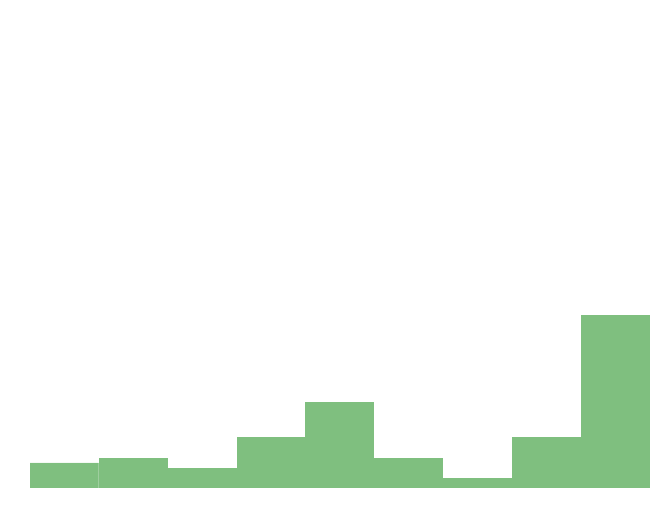
\includegraphics[width = 2cm, height = 0.5cm]{tex-inputs/table-images/internetben} \\ 
Electricity & 88.0 & 50.0 & 100.0 & 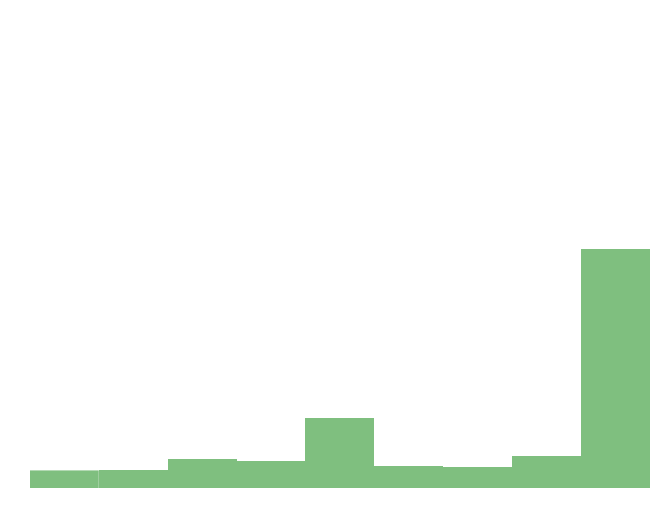
\includegraphics[width = 2cm, height = 0.5cm]{tex-inputs/table-images/ElectricityBenefit} \\ 
\hline
\end{tabular}
\caption{Benefit rankings in response to the Fischoff-style prompt for various technologies and capabilities. Most technologies are capabilities with respect to wearable devices. Calibration technologies were electricity, guns, lawnmowers, and motorcycles. Wearable technologies included the Google Glass and the Cubetastic3000. Other specific technologies, such as internet, email, laptops, and smartphones, were also asked. }
\label{benefit}
\end{center}
\end{table}